\documentclass[aspectratio=149]{beamer}

\usepackage[utf8]{inputenc}
\usepackage[T1]{fontenc}

\usepackage[english]{babel}
\usepackage{amsmath}
\usepackage{cleveref}
\usepackage{amssymb}
\usepackage{mathtools}

%%Numbers, expectation
\newcommand{\N}{\mathbb{N}}
\newcommand{\E}{\mathbb{E}}
\renewcommand{\P}{\mathbb{P}}
\newcommand{\Var}{\mathbb{V}}
\newcommand{\R}{\mathbb{R}}
\newcommand{\D}{\mathcal{D}}
\newcommand{\B}{\mathcal{B}}
\newcommand{\Dh}{\D_h}
\renewcommand{\phi}{\varphi}
\newcommand*\diff{\mathop{}\!\mathrm{d}} % integral

%% mathoperator
\DeclareMathOperator*{\argmax}{arg\,max}
\DeclareMathOperator*{\argmin}{arg\,min}
\DeclareMathOperator*{\dom}{dom}
\DeclareMathOperator*{\sign}{sign}
\DeclareMathOperator*{\diag}{diag}

\DeclareMathOperator*{\Cov}{Cov}
\DeclareMathOperator*{\Cor}{Corr}
\DeclareMathOperator*{\Id}{Id}

%proximal operator
\newcommand{\prox}[3][]{\operatorname{prox}^{#1}_{#2}\left(#3 \right)}

\usepackage{xcolor}

%% sort citations by increasing number
\usepackage[sort,nocompress]{cite}

\usepackage{graphicx}% http://ctan.org/pkg/graphicx
\graphicspath{{../figures/}{../../figures}{../../memes}} %Setting the graphicspath
\usepackage{caption,subcaption}

\usepackage{tikz}
\usepackage{pgfplots}
\usetikzlibrary{backgrounds}
\usetikzlibrary{intersections}
\usepgfplotslibrary{fillbetween}

% \usepackage[right]{showlabels}


%%
\theoremstyle{plain}
\newtheorem{prop}{Proposition}[section]
\newtheorem{algo}{Algorithm}[section]
\newtheorem{assumption}{Assumption}
\theoremstyle{remark}
\newtheorem{remark}{Remark}[section]

% cref
\crefname{assumption}{Assumption}{Assumptions}
\crefname{equation}{}{}

\usepackage{autonum}

\usepackage{bm} %% bold math symbols

\usepackage{bbm} %% for \mathbbm{1}


% algorithmic environment
\usepackage{algorithm}
\usepackage[noend]{algpseudocode}

% for some reason this was required on one void linux installation (but not the other)
\usepackage{sansmathaccent}
\pdfmapfile{+sansmathaccent.map}

\author{Axel Böhm}

% shows which section we're in
\usetheme{Darmstadt}

% page number
\setbeamertemplate{footline}[frame number]
\setbeamercolor{page number in head/foot}{fg=gray}


% display things like onslide or visible already before but grayed out
\setbeamercovered{transparent}

% set the itemize item symbol as a diamond
\setbeamertemplate{itemize item}{$\diamond$}
% set the itemize subitem symbol as a triangle
\setbeamertemplate{itemize subitem}{$\blacktriangleright$}

% set the enumerate item symbol as a roman numbers
\setbeamertemplate{enumerate item}{(\roman{enumi})}


\author{Axel Böhm}

% shows which section we're in
\usetheme{Darmstadt}

% page number
\setbeamertemplate{footline}[frame number]
\setbeamercolor{page number in head/foot}{fg=gray}


% display things like onslide or visible already before but grayed out
\setbeamercovered{transparent}

% set the itemize item symbol as a diamond
\setbeamertemplate{itemize item}{$\diamond$}
% set the itemize subitem symbol as a triangle
\setbeamertemplate{itemize subitem}{$\blacktriangleright$}

% set the enumerate item symbol as a roman numbers
\setbeamertemplate{enumerate item}{(\roman{enumi})}


% reference: https://yuxinchen2020.github.io/ele522_optimization/lectures/variance_reduction.pdf
% or
% https://ieeexplore-ieee-org.uaccess.univie.ac.at/stamp/stamp.jsp?tp=&arnumber=9226504

\usepackage{booktabs}

\title{Variance reduction for stochastic gradient methods}
\date{\today}

\begin{document}
\maketitle
\frame{\tableofcontents}


\section{Introduction}%

\begin{frame}
  \frametitle{The finite sum probem}
  A common Task in (supervised) machine learning:
  \begin{equation}
    \min_{x\in \R^d} f(x) := \frac{1}{n} \sum_{i=1}^{n} \underbrace{f_i(x)}_{\textcolor{blue}{\text{loss for $i$-th sample}}} + \underbrace{\psi(x)}_{\textcolor{blue}{\text{regularizer}}}
  \end{equation}
  where the $i$-th sample is $(a_i, y_i)$.

  \textbf{Examples:}
  \begin{itemize}
    \item linear regression: $f_i(x) = {(a_i^T x -y_i)}^2$, and $\psi=0$
    \item logistic regression: $f_i(x) = \log(1+e^{-y_i a_i^T x})$, and $\psi=0$
          ``sigmoid function'' and logistic loss.
    \item Lasso: $f_i$ as for linear regression but $\psi(x) = \Vert x \Vert_1$
    \item SVM: $f_i(x) = \max \{0 , 1 - y_i a_i^T x\}$ and $\psi(x)= \Vert x \Vert^2$
  \end{itemize}
\end{frame}

\begin{frame}
  \frametitle{Gradient descent}
  \begin{algorithm}[H]
    \caption{(batch) GD}
    \begin{algorithmic}[1]
      \For{$k = 1,2, \dots$}
      \State{ $x_{k+1} = x_k  - \alpha_k \nabla f(x_k) $}
      \EndFor{}
    \end{algorithmic}
  \end{algorithm}

  \begin{itemize}
    \item gradient can be computed via
          \begin{equation}
            \nabla f(x) = \nabla \left(\sum_{i=1}^{n}f_i(x)\right) = \sum_{i=1}^{n} \nabla f_i(x_k)
          \end{equation}
    \item good convergence properties
    \item can be \textbf{expensive} if $n$ is large!
  \end{itemize}
\end{frame}


\begin{frame}
  \frametitle{Stochastic gradient descent}
  \begin{algorithm}[H]
    \caption{SGD}\label{sgd}
    \begin{algorithmic}[1]
      \For{$k = 1,2, \dots$}
      \State{pick $i_k$ uniform at random in $[n]$}
      \State{$x_{k+1} = x_k  - \alpha_k \nabla f_{i_k}(x_k)$}
      \EndFor{}
    \end{algorithmic}
  \end{algorithm}

  We already noticed that:
  \begin{itemize}
    \item unbiased: $\E[\nabla f_{i_k}(x)] = \sum_{i=1}^{n} \P[i=i_k] \nabla f_i(x) = \sum_{i=1}^{n} \frac{1}{n} \nabla f_i(x)$
    \item large stepsizes fail to suppress noise in the stoch.\ gradients \\
          $\rightarrow$ leads to oscillations
    \item decreasing stepsizes mitigate this problem but \textbf{slows down} convergence (too \emph{conservative})
  \end{itemize}

\end{frame}


\begin{frame}
  \frametitle{Recall SGD}
  \begin{block}{template}
    \begin{equation}
      x_{k+1} = x_k - \alpha_k g_k
    \end{equation}
  \end{block}
  \begin{itemize}
    \item $g_k$ is an unbiased estimator of the true gradient $\nabla F(x_k)$
    \item convergence depends on \textbf{variance} $\E [ \Vert g_k - \nabla F(x_k) \Vert ] \le \sigma_g$ \\
          (not strictly necessary)
    \item vanilla SGD uses $g_k = \nabla f_{i_k}(x_k)$ \\
          \textbf{issue:} $\sigma_g$ is non-negligible even close to the solution
    \item \textbf{Q:} can we choose $g_k$ in a different way to reduce variability?
  \end{itemize}

\end{frame}

\begin{frame}
  \frametitle{Minibatching}
  \begin{algorithm}[H]
    \caption{minibatch SGD}
    \begin{algorithmic}[1]
      \For{$k = 1,2, \dots$}
      \State{pick $I_k$ random subset of $[n]$ with $\vert I_k \vert = b $}
      \State{$x_{k+1} = x_k  - \alpha_k \sum_{i \in I_k} \nabla f_{i}(x_k)$}
      \EndFor{}
    \end{algorithmic}
  \end{algorithm}
  \begin{itemize}
    \item typically we make a (uniform) \emph{random} choice $i_k \in [n] = \{1, \dots, n\}$\\
          (or random reshuffling)
    \item by increasing the size to a \textbf{random subset} $I_k \subset [n]$ of size $b \ll n$ we can
          \begin{itemize}
            \item decrease variance
            \item increase cost only moderately,
            \item no improvement in the rate
          \end{itemize}
  \end{itemize}

\end{frame}


\begin{frame}
  \frametitle{A simple idea}
  Consider
  \begin{itemize}
    \item estimator $X$ for parameter $\mu$ ($\E[X]=\mu$ and $\Var[X]=\sigma^2$)
    \item want to \textcolor{blue}{keep unbiased} but \textbf{\textcolor{blue}{reduce variance}}
    \item find $Y$ such that $\E[Y] = 0$ but $\Cov (X,Y)$ \textbf{is large} and define
          \begin{equation}
            \tilde{X} := X-Y
          \end{equation}
    \item remains unbiased
    \item $\Var[\tilde{X}]$ can be much smaller than $\Var[X]$ if $X,Y$ are highly correlated
          \begin{equation}
            \Var[\tilde{X}] = \Var[X]+\Var[Y]-2\Cov[X,Y]
          \end{equation}
  \end{itemize}
\end{frame}

\section{SAG}%
\label{sec:}

\begin{frame}
  \frametitle{Stochastic average gradient (SAG), 2013}
  \begin{itemize}
    \item \textbf{maintain table} containing gradients $g_i$ of $f_i$
    \item pick random $i_k \in [n]$ and
          \begin{equation}
            g_{i_k}^k := \nabla f_{i_k}(x^{k})
          \end{equation}
          set $g_{i}^k = g_i^{k-1}$ for all $i\neq i_k$ (remain the same)
    \item Update
          \begin{equation}
            x^{k+1} = x^k - \alpha_k \frac{1}{n} \sum_{i=1}^{n} g_i^k.
          \end{equation}
    % \item assuming gradients do not change too much along trajectory
    \item gradient estimator \textcolor{red}{no longer unbiased}
    \item Isn't it expensive to average these gradients?
          \begin{equation}
            x^{k+1} = x^k -u \alpha_k  \Big( \frac{g_{i_k}^k}{n} - \frac{g_{i_k}^{k-1}}{n} + \underbrace{\frac{1}{n}\sum_{i=1}^{n} g_i^{k-1}}_{\text{old table average}} \Big)
          \end{equation}
  \end{itemize}
\end{frame}


\begin{frame}
  \frametitle{SAG variance reduction}
  Gradient estimator in SAG:
  \begin{equation}
    x^{k+1} = x^k - \alpha_k \frac{1}{n} \Big( \underbrace{g_{i_k}^k}_X - \underbrace{g_{i_k}^{k-1} - \sum_{i=1}^{n} g_i^{k-1}}_{Y} \Big)
  \end{equation}
  \begin{itemize}
    \item Indeed $\E[X] = \nabla f(x^k)$, but $\E[Y]\neq 0$ $\rightarrow $ is \textbf{biased estimator}
    \item $X$ and $Y$ are correlated as $X-Y \to 0$:
          \begin{itemize}
            \item $x^k$ and $x_{k-1}$ both converge to $x^*$ $\Rightarrow$ $ \nabla f_i(x_k) - \nabla f_i(x_{k-1}) \to 0$
            \item the last term converges to $\nabla f(x^*)= 0$
          \end{itemize}
  \end{itemize}
\end{frame}

\begin{frame}
  \frametitle{Convergence}
  As always, initialization plays a role: $D^2 := \Vert x^0 -x^* \Vert^2$.

  \begin{equation}
    \begin{aligned}
      \text{SAG:}& \quad \frac{n}{k}(f(x^0)-f^*) + \frac{L}{k}D^2 \\
      \text{GD:}& \quad \frac{L}{k}D^2 \\
      \text{SGD:}& \quad \frac{L}{\sqrt{k}}D^2 \\
    \end{aligned}
  \end{equation}
  \begin{itemize}
    \item Achieves \textcolor{blue}{linear convergence} in the \textbf{strongly} convex setting.
    \item proofs are difficult (and computer-aided)
  \end{itemize}


  \begin{center}
    Same gradient oracle cost as SGD, but same converge rate as GD.
  \end{center}
\end{frame}


\begin{frame}
  \frametitle{Experiments from the original paper}
  \begin{figure}[ht]
    \centering
    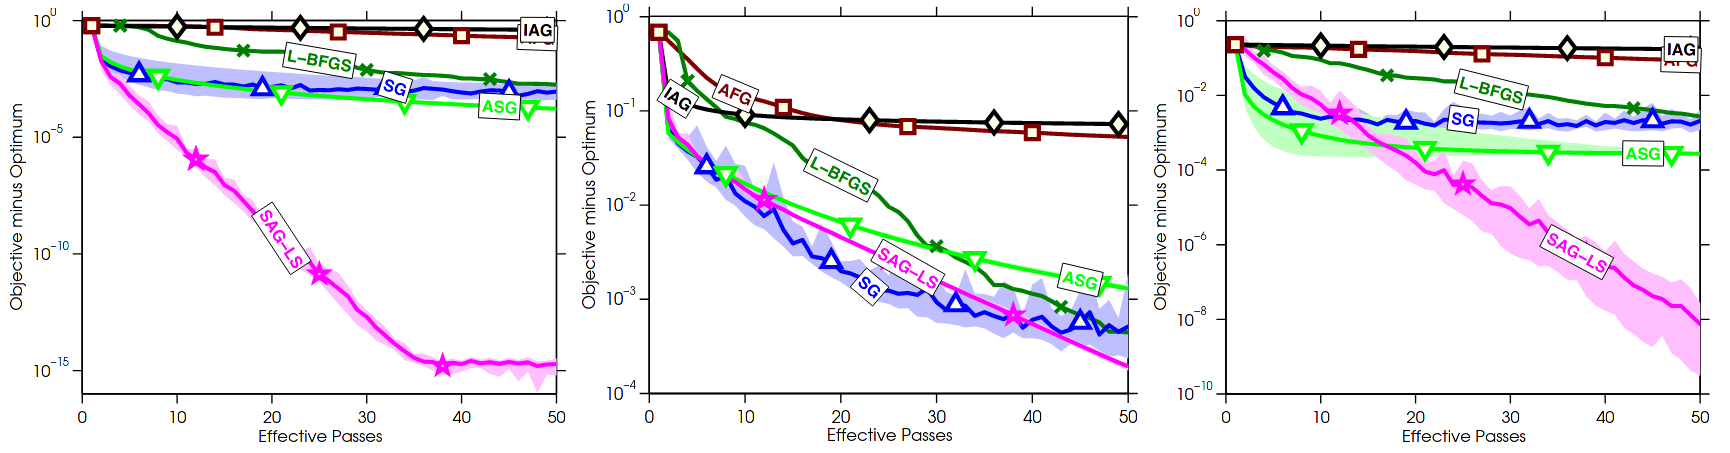
\includegraphics[width=\textwidth,height=\textheight,keepaspectratio]{SAG-experiments}
    \caption{ Solving $\ell_2$-regularized logistic regression.}
  \end{figure}
\end{frame}


\begin{frame}
  \frametitle{More ``naive'' implementation}
  \begin{figure}[ht]
    \centering
    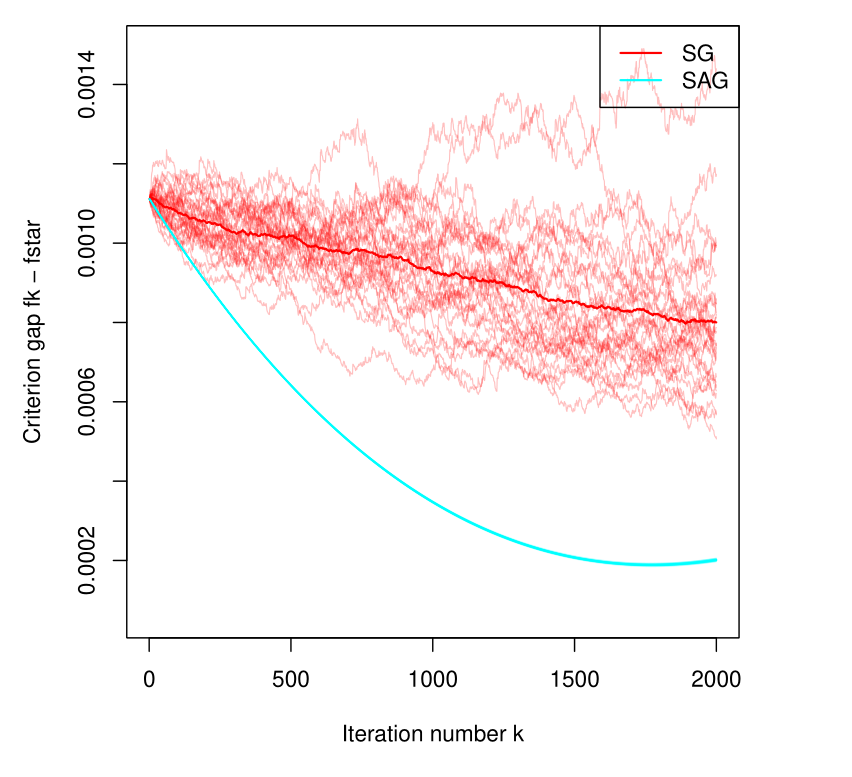
\includegraphics[width=\textwidth,height=0.9\textheight,keepaspectratio]{SAG}
  \end{figure}
\end{frame}


\begin{frame}
  \frametitle{SAG experiments}
  \begin{itemize}
    \item does not work well out of the box
    \item needs a \textcolor{blue}{warm up} to get good $(g_1^0, g_2^0, \dots, g_m^0)$
          \begin{itemize}
            \item achieved by running one full epoch of SGD
          \end{itemize}
    \item reguires hand tuned stepsize or line search
  \end{itemize}

\end{frame}


\section{SAGA}%
\label{sec:}

\begin{frame}
  \frametitle{SAGA, 2014}
  Very similar to SAG:
  \begin{itemize}
    \item maintain table containing gradients $g_i$ of $f_i$
    \item pick random $i_k \in [n]$ and
          \begin{equation}
            g_{i_k}^k := \nabla f_{i_k}(x^{k})
          \end{equation}
          set $g_{i}^k = g_i^{k-1}$ for all $i\neq i_k$ (remain the same)
    \item Update
          \begin{equation}
            x^{k+1} = x^k - \alpha_k  \Big( g_{i_k}^k - g_{i_k}^{k-1} + \frac{1}{n}\sum_{i=1}^{n} g_i^k \Big)
          \end{equation}
    \item estimator now \textbf{unbiased}!
  \end{itemize}
\end{frame}

\begin{frame}
  \frametitle{For Comparison}
  SAGA gradient estimate:
  \begin{equation}
    g_{i_k}^k - g_{i_k}^{k-1} + \frac{1}{n}\sum_{i=1}^{n} g_i^k.
  \end{equation}

  SAG gradient estimate:
  \begin{equation}
    \frac{1}{n}g_{i_k}^k - \frac{1}{n}g_{i_k}^{k-1} + \frac{1}{n}\sum_{i=1}^{n} g_i^k.
  \end{equation}
\end{frame}


\begin{frame}
  \frametitle{Experiments from the original paper}
  \begin{figure}[ht]
    \centering
    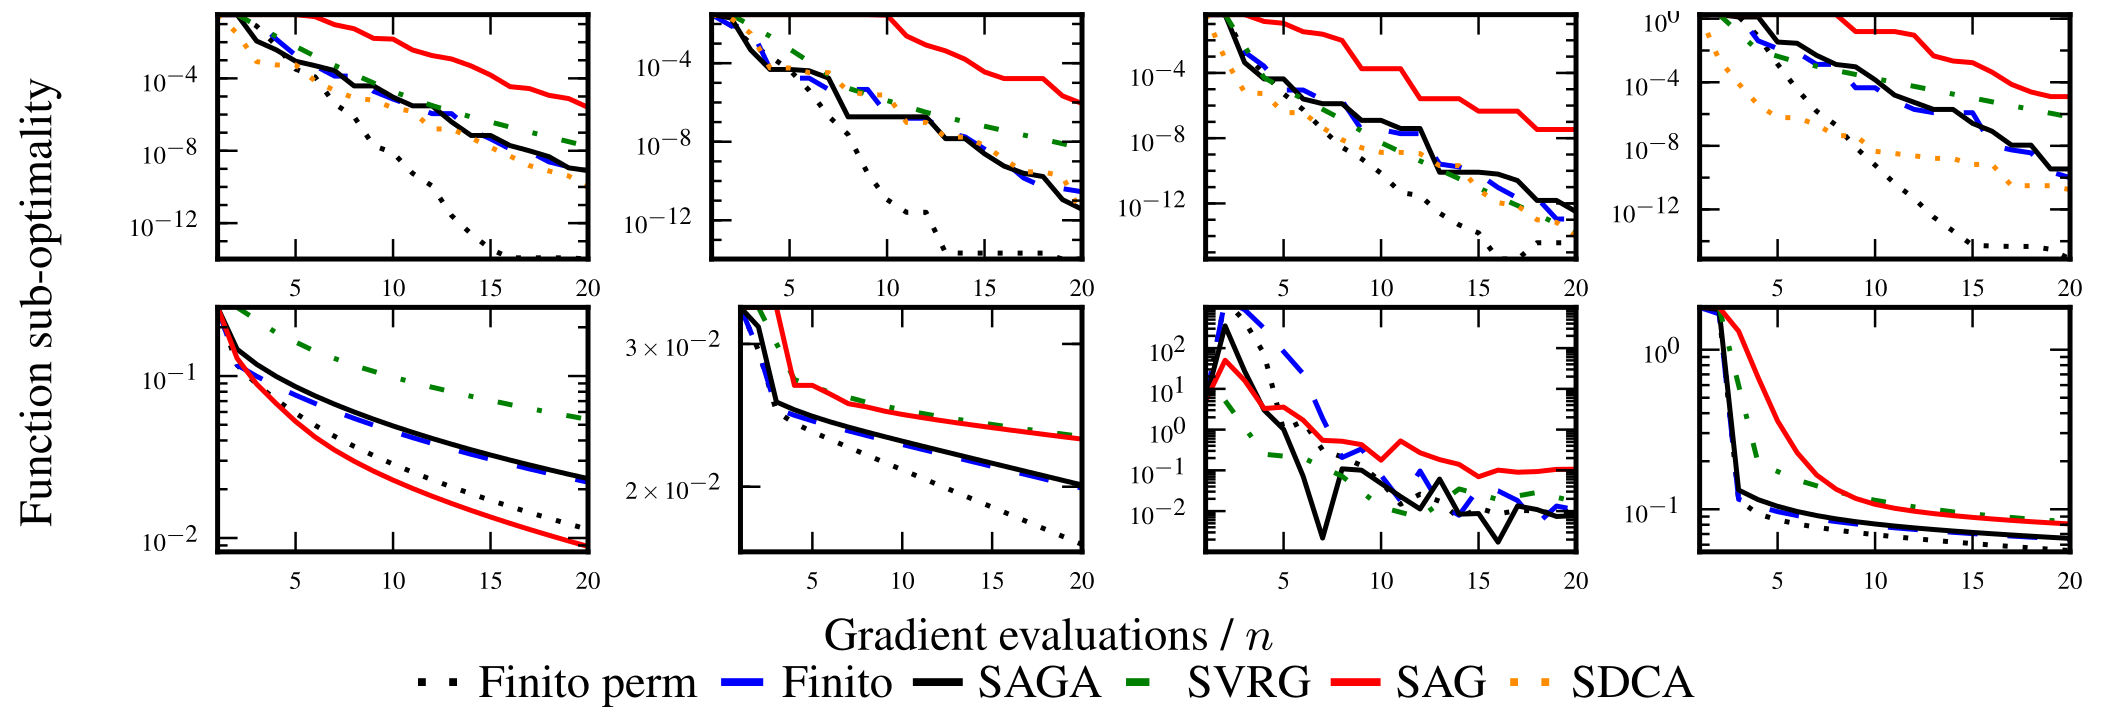
\includegraphics[width=\textwidth,height=\textheight,keepaspectratio]{SAGA-experiments}
    \caption{Solving regularized logistic regression. First row is $\ell_2$-regularized; second row is $\ell_1$.}
  \end{figure}
\end{frame}


\begin{frame}
  \frametitle{More ``naive'' implementation}

  \begin{figure}[ht]
    \centering
    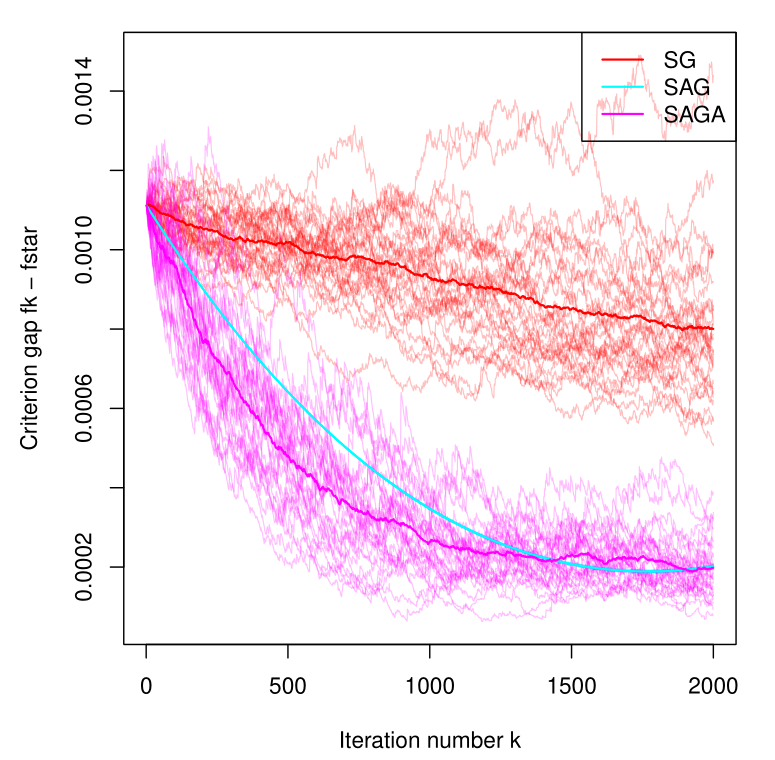
\includegraphics[width=\textwidth,height=0.9\textheight,keepaspectratio]{SAGA.png}
    \caption{Highlights the low variance of SAG.}
  \end{figure}
\end{frame}


\section{SVRG}%

\begin{frame}
  \frametitle{Stochastic Variance Reduced Gradient (SVRG), 2013}

  \begin{algorithm}[H]
    \caption{SVRG}\label{}
    \begin{algorithmic}[1]
      \For{$k=1,2, \dots$}
      \State{Set $x^1 = \tilde{x} = \tilde{x}^{k}$}
      \State{Compute $\tilde{\mu} := \nabla f(\tilde{x})$ \hfill \textcolor{blue}{//update snapshot}}
      \For{$l=1,2, \dots, m$ }\hfill \textcolor{blue}{//$m$ iterations per epoch}
      \State{pick $i_l$ uniform at random in $[n]$}
      \State{Set $x^{l+1} = x^l - \alpha (\nabla f_{i_l}(x^l) - \nabla f_{i_l}(\tilde{x}) + \tilde{\mu})$}
      \EndFor{}
      \State{$\tilde{x}^{k+1}= x^{m+1}$}
      \EndFor{}
    \end{algorithmic}
  \end{algorithm}
  \begin{itemize}
    \item Does \textbf{\textcolor{blue}{not need to store}} full table of gradients.
    \item requires \emph{batch} gradient computation every \emph{epoch}
    \item per iteration cost is comparable to that of SGD if $m \ge n$
    \item convergence rates similar to SAGA, but simpler analysis.
  \end{itemize}
\end{frame}

\begin{frame}
  \frametitle{SVRG}
  \textbf{key idea:} by storing old point we can
  \begin{equation}
    \underbrace{\nabla f_{i_k}(x^k) - \nabla f_{i_k}(x^{\text{old}})}_{\text{$\to 0$ if $x\approx x^{\text{old}}$}} + \underbrace{\nabla f(x^{\text{old}})}_{\text{$\to 0$ if $x^{\text{old}}$}}
  \end{equation}
  \begin{itemize}
    \item is an unbiased estimate of $\nabla f(x^k)$
    \item converges to $0$ (meaning reduced variability) if $x^k\approx x^{\text{old}} \approx x^*$
  \end{itemize}

\end{frame}

\begin{frame}
  \frametitle{SVRG: Theorem}

  \textcolor{gray}{Each $f_i$ is convex and $L$-smooth, and sum is $\mu$-strongly convex.}

  \begin{theorem}
    Choose $m$ large enough s.t. $\rho = \frac{1}{\mu \alpha (1-2L \alpha)m} + \frac{2L \alpha}{1-2L \alpha}< 1$, then
    \begin{equation}
      \E[F(x_s^{old})- F(x^*)] \le \rho^s [F(x_0^{old})-F(x^*)]
    \end{equation}
  \end{theorem}
  Computational cost:
  \begin{itemize}
    \item per epoch: $(m+n)$
    % \item complexity: $(n+ \kappa) \log(1/\epsilon)$
    \item inner loop is annoying (has to choose $m$) $\rightarrow$ loopless variant
  \end{itemize}
\end{frame}

\begin{frame}
  \frametitle{SVRG: Convergence Proof}
  Denote $g_s^k = \nabla f_{i_l}(x_s^k) - \nabla f_{i_l}(x_s^{old}) + \nabla F(x_s^{old})$. Conditioning on everything prior to $x_s^{k+1}$ we get
  \begin{equation}
    \begin{aligned}
      \MoveEqLeft \E [\Vert x_s^{k+1} - x^* \Vert^2] = \E [\Vert x_s^{k}- \alpha g_s^k - x^* \Vert^2] \\
      &= \Vert x_s^k-x^* \Vert^2 - 2 \alpha {(x_s^k-x^* )}^T \E[g_s^t] + \alpha^2 \E[\Vert g_s^k \Vert^2] \\
      &= \Vert x_s^k-x^* \Vert^2 - 2 \alpha {(x_s^k-x^* )}^T \textcolor{blue}{\nabla F(x_s^t)} + \alpha^2 \E[\Vert g_s^k \Vert^2] \\
      &\le \Vert x_s^k-x^* \Vert^2 - 2 \alpha (F(x_s^k) - F(x^*))+ \alpha^2 \E[\Vert g_s^k \Vert^2]
    \end{aligned}
  \end{equation}

  \begin{itemize}
     \item \textbf{key step:} control $\E[\Vert g_s^k \Vert^2]$
   \end{itemize}
\end{frame}

\begin{frame}
  \frametitle{SVRG: convergence Proof}
  \begin{lemma}%
    \begin{equation}
      \E[\Vert g_s^k \Vert^2] \le 4L [ F(x_s^k)- F(x^*) + F(x_s^{old}-F(x^*)) ]
    \end{equation}

  \end{lemma}

\end{frame}


\begin{frame}
  \frametitle{Comparison}

  % \begin{tabular}{l | c}
  %   SVRG & $(n + \kappa) \log(1/\epsilon)$\\
  %   GD   & $n \kappa \log(1/\epsilon)$ \\
  %   SGD  & $\kappa^2 / \epsilon$
  % \end{tabular}

  % \textbf{\textcolor{blue}{Strongly convex}} problems: number gradient calls to compute:
  % \begin{equation}
  %   \E [f(x_k)] - f^* \le \epsilon
  % \end{equation}
  % is given by
  \textbf{\textcolor{blue}{Strongly convex}} problems: number gradient calls to compute $\E [f(x_k)] - f^* \le \epsilon$ is given by
  \begin{center}
    \begin{tabular}{c c c}
      SVRG / SAGA  & GD & SGD \\
      \midrule
      $(n + \kappa) \log \frac{1}{\epsilon}$ & $n \kappa \log \frac{1}{\epsilon}$ & $\kappa^2 / \epsilon$
    \end{tabular}
  \end{center}
  \vspace{1cm}
  \begin{figure}[ht]
    \centering
    \includegraphics[width=\textwidth,height=\textheight,keepaspectratio]{SAGA-table-comparison}
    \caption{Summary of other relevant properties.}
  \end{figure}

  % \begin{itemize}
  %   \item SVRG:\ $(n + \kappa) \log(1/\epsilon)$
  %   \item GD:\ $n \kappa \log(1/\epsilon)$
  %   \item SGD:\ $\kappa^2 / \epsilon$
  % \end{itemize}

\end{frame}

\section{Katyusha}%
\label{sec:}

\begin{frame}
  \frametitle{Variance reduction + momentum/acceleration}
  \begin{block}{}
    \centering
    \textbf{Katyusha}
  \end{block}

  \textbf{\textcolor{blue}{Strongly convex}} problems: number gradient calls to compute $\E [f(x_k)] - f^* \le \epsilon$ is given by
  \begin{center}
  \begin{tabular}{c c c c c}
    Katyusha & SVRG / SAGA  & GD & NAG & SGD \\
    \midrule
    $(n + \sqrt{n \kappa}) \log \frac{1}{\epsilon}$ &$(n + \kappa) \log \frac{1}{\epsilon}$ & $n \kappa \log \frac{1}{\epsilon}$ & $n \sqrt{\kappa} \log \frac{1}{\epsilon}$ & $\kappa^2 / \epsilon$
  \end{tabular}
  \end{center}
  \vspace{1cm}
  \begin{itemize}
    \item Improvement critical for \textbf{\textcolor{blue}{ill conditioned}} ($\kappa \gg n$) problems.
  \end{itemize}


\end{frame}


\begin{frame}
  \frametitle{Katyusha in the non-strongly convex setting}
  \textbf{\textcolor{blue}{just convex}} problems: number gradient calls to compute $\E [f(x_k)] - f^* \le \epsilon$ is given by
  \begin{center}
  \begin{tabular}{c c c c c c}
    lower bound & Katyusha & SVRG / SAGA  & GD & NAG & SGD \\
    \midrule
    $n + \sqrt{\frac{n L}{\epsilon}}$ & $n \log \frac{1}{\epsilon} + \sqrt{\frac{n L}{\epsilon}}$ &$\frac{L}{\epsilon}$ & $n \frac{L}{\epsilon}$ & $n \sqrt{\frac{L}{\epsilon}}$ & $ \frac{1}{\sqrt{\epsilon}}$
  \end{tabular}
  \end{center}
  \vspace{1cm}
  \textcolor{gray}{Almost matches lower bound.}

\end{frame}


\begin{frame}
  \frametitle{Summary}

  \begin{itemize}
    \item Variance reduction recovers the rates of batch (deterministic methods)
    \item but (more or less) keeps number of gradient calls of SGD
    \item still require batch gradient computations sometimes
    \item requires offline setting (multiple passes through data)
    \item requires knowledge of (multiple) parameters to get good stepsize
  \end{itemize}

  \textcolor{gray}{
  Check out this fantastic review paper:
  https://ieeexplore-ieee-org.uaccess.univie.ac.at/stamp/stamp.jsp?tp=&arnumber=9226504}

\end{frame}



\end{document}
